\ac{CNN}s are neural networks using convolutional layers. Convolutional layers are designed to input multidimensional arrays and output multidimensional arrays. 
%
For image classification, the input is composed of one or more two-dimensional arrays called channels. The channels share the same shape $w_{in} \times h_{in}$.
Consequently, the input can be represented as a three-dimensional array of shape $w_{in} \times h_{in} \times d_{in}$ with $d_{in}$ being the number of channels.
%
The output is composed of one or more two-dimensional arrays called feature maps. The feature maps share the same shape $w_{out} \times h_{out}$. Consequently, the output can be represented as a three-dimensional array of shape $w_{out} \times h_{out} \times d_{out}$ with $d_{out}$ being the number of feature maps. \autocites{LeCun.2015b}{LeCun.1998}
This is illustrated in Figure \ref{fig:cnnlayer}.
\begin{figure}[H]
	\centering
	%\cube{x offset}{y offset}{width}{height}{depth}{color}{fillcolor}

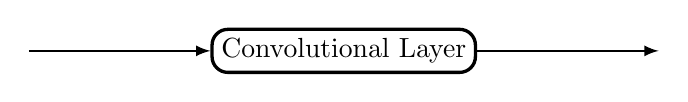
\begin{tikzpicture}[
cell/.style={
	rectangle, 
	rounded corners=2mm, 
	draw,
	very thick,
	align=center,
},
ArrowC1/.style={% Arrows with rounded corners
	rounded corners=.25cm,
	thick,
},
]
\cube{0}{0}{1}{4}{4}{black}{gray}
\node[cell] (layer) at (4,-2,-2) {Convolutional Layer};
\cube{9}{0}{1}{4}{4}{black}{gray}

\draw[-latex,ArrowC1] (0,-2,-2) -- (layer);
\draw[-latex,ArrowC1] (layer) -- (8,-2,-2);

\end{tikzpicture}
	\caption{Convolutional Layer (own figure)} \label{fig:cnnlayer}
\end{figure}
\par
Convolutional layers consist of neurons which only connect to a small region of the layer's input, see Figure \ref{fig:cnnneuron}. This region is called receptive field\autocite{LeCun.1998}. Within a receptive field, each connection of a neuron is connected to one element of the input. Consequently, a receptive field can be seen as an array slice of the layer's input. This array is of shape $k \times k \times d$.
The set of weights of a convolutional neuron's connections is referred to as filter or kernel.
The kernel can be represented as a three-dimensional array of shape $k \times k \times d$. $k$ is the size of the kernel. \autocites{Rawat.2017}{LeCun.2015b}
\par
A convolutional layer holds one neuron for each receptive field and for each kernel. This means, neurons of the same kernel share the same weights. On that account, neurons of the same kernel can be seen as $r$ copies of a neuron connected to all receptive fields or applying the same neuron to each receptive field. Applying the same neuron to each receptive field can be imagined as sliding the neuron over the input. The output of a neuron is computed as described in Section \ref{sec:neuralnetwork}. Given the input $X$, a kernel $K$, and the receptive field $X[i:i+k, j:j+k]$, the output of a neuron $y$ is computed as defined by Equation \eqref{eq:convneuron}. As a result, the output of all neurons of a kernel is computed by computing the output for all receptive fields with $i \in \{x|x_0=0, x \le w-k, x_{n+1} = x_n+stride\}$ and $j \in \{x|x_0=0, x \le h-k, _{n+1} = x_n+stride\}$. This computation loosely relates to discrete convolution. For this reason, \ac{CNN}s are called convolutional. The resulting output is a feature map. Hence, the output of a convolutional layer is computed by computing all feature maps. Derived from this, the shape of the output is $\frac{w-k+2 \cdot padding}{stride}+1 \times \frac{h-k+2 \cdot padding}{stride}+1 \times k$. Padding can be described as increasing  the input's width and height by $padding$ on both sides by filling with zeros. Imagining sliding the neuron over the input, $stride$ is the step size by which the neuron is slid. \autocite{Goodfellow.2016}
\begin{equation}
	\label{eq:convneuron}
	y = \varphi(\sum X[i:i+k, j:j+k] \cdot K)
\end{equation}
\begin{figure}[H]
	\centering
	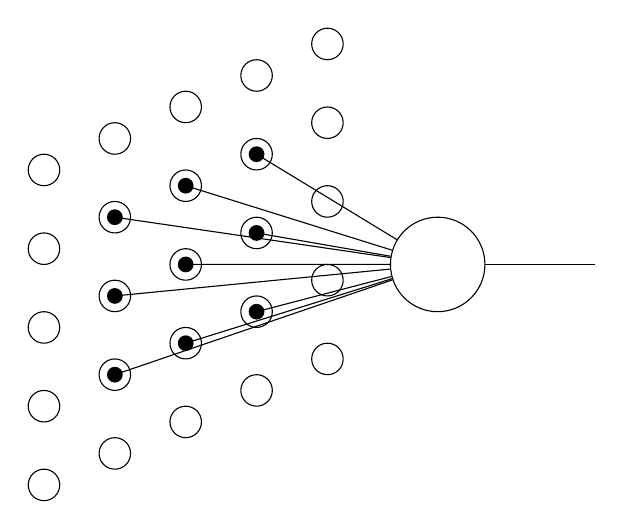
\begin{tikzpicture}
				\node[draw, circle, minimum size=1.2cm] (n) at (5,2.8) {};
				\draw (n) --  (7,2.8);
				\foreach \x in {0,1,2,3,4}
					\foreach \y in {0,1,2,3,4}
						\draw (\x*0.9+ \y*0, \x*0.4+\y*1) circle (0.2cm); %Matrixtransformation (0.7 0; 0.3 1)
				\foreach \x in {1,2,3}
					\foreach \y in {1,2,3} {
						\draw (\x*0.9+ \y*0, \x*0.4+\y*1) -- (n);
						\fill (\x*0.9+ \y*0, \x*0.4+\y*1) circle (0.1cm);
					}
			\end{tikzpicture}
	\caption{Neuron of a Convolutional Neural Network (own figure)} \label{fig:cnnneuron}
\end{figure}
\par 
For better understanding, convolution, stride, and padding are illustrated in the following paragraphs. 
\paragraph{Convolution}For example, consider the case of a grayscale image represented as one channel $X$, a kernel $K$, and an identity activation function $\varphi$. Then, the output of a convolutional neuron is computed by laying the kernel on top of the channel. Each value of the activation map is computed by multiplying the overlapping values. The resulting values are summed. The sum is processed by the activation function. In this case, the activation function is the identity function. Thus, the result is the sum itself. The activation map $Y$ is computed by sliding the kernel over each row and each column by the factor of stride. This is illustrated in Figure \ref{fig:conv}.\autocite{Goodfellow.2016}
\begin{figure}[H]
	\centering
	\ac{CNN}s are neural networks using convolutional layers. Convolutional layers are designed to input multidimensional arrays and output multidimensional arrays. 
%
For image classification, the input is composed of one or more two-dimensional arrays called channels. The channels share the same shape $w_{in} \times h_{in}$.
Consequently, the input can be represented as a three-dimensional array of shape $w_{in} \times h_{in} \times d_{in}$ with $d_{in}$ being the number of channels.
%
The output is composed of one or more two-dimensional arrays called feature maps. The feature maps share the same shape $w_{out} \times h_{out}$. Consequently, the output can be represented as a three-dimensional array of shape $w_{out} \times h_{out} \times d_{out}$ with $d_{out}$ being the number of feature maps. \autocites{LeCun.2015b}{LeCun.1998}
This is illustrated in Figure \ref{fig:cnnlayer}.
\begin{figure}[H]
	\centering
	%\cube{x offset}{y offset}{width}{height}{depth}{color}{fillcolor}

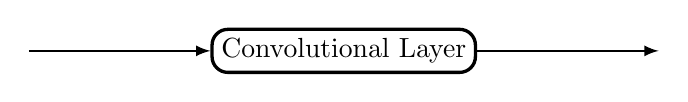
\begin{tikzpicture}[
cell/.style={
	rectangle, 
	rounded corners=2mm, 
	draw,
	very thick,
	align=center,
},
ArrowC1/.style={% Arrows with rounded corners
	rounded corners=.25cm,
	thick,
},
]
\cube{0}{0}{1}{4}{4}{black}{gray}
\node[cell] (layer) at (4,-2,-2) {Convolutional Layer};
\cube{9}{0}{1}{4}{4}{black}{gray}

\draw[-latex,ArrowC1] (0,-2,-2) -- (layer);
\draw[-latex,ArrowC1] (layer) -- (8,-2,-2);

\end{tikzpicture}
	\caption{Convolutional Layer (own figure)} \label{fig:cnnlayer}
\end{figure}
\par
Convolutional layers consist of neurons which only connect to a small region of the layer's input, see Figure \ref{fig:cnnneuron}. This region is called receptive field\autocite{LeCun.1998}. Within a receptive field, each connection of a neuron is connected to one element of the input. Consequently, a receptive field can be seen as an array slice of the layer's input. This array is of shape $k \times k \times d$.
The set of weights of a convolutional neuron's connections is referred to as filter or kernel.
The kernel can be represented as a three-dimensional array of shape $k \times k \times d$. $k$ is the size of the kernel. \autocites{Rawat.2017}{LeCun.2015b}
\par
A convolutional layer holds one neuron for each receptive field and for each kernel. This means, neurons of the same kernel share the same weights. On that account, neurons of the same kernel can be seen as $r$ copies of a neuron connected to all receptive fields or applying the same neuron to each receptive field. Applying the same neuron to each receptive field can be imagined as sliding the neuron over the input. The output of a neuron is computed as described in Section \ref{sec:neuralnetwork}. Given the input $X$, a kernel $K$, and the receptive field $X[i:i+k, j:j+k]$, the output of a neuron $y$ is computed as defined by Equation \eqref{eq:convneuron}. As a result, the output of all neurons of a kernel is computed by computing the output for all receptive fields with $i \in \{x|x_0=0, x \le w-k, x_{n+1} = x_n+stride\}$ and $j \in \{x|x_0=0, x \le h-k, _{n+1} = x_n+stride\}$. This computation loosely relates to discrete convolution. For this reason, \ac{CNN}s are called convolutional. The resulting output is a feature map. Hence, the output of a convolutional layer is computed by computing all feature maps. Derived from this, the shape of the output is $\frac{w-k+2 \cdot padding}{stride}+1 \times \frac{h-k+2 \cdot padding}{stride}+1 \times k$. Padding can be described as increasing  the input's width and height by $padding$ on both sides by filling with zeros. Imagining sliding the neuron over the input, $stride$ is the step size by which the neuron is slid. \autocite{Goodfellow.2016}
\begin{equation}
	\label{eq:convneuron}
	y = \varphi(\sum X[i:i+k, j:j+k] \cdot K)
\end{equation}
\begin{figure}[H]
	\centering
	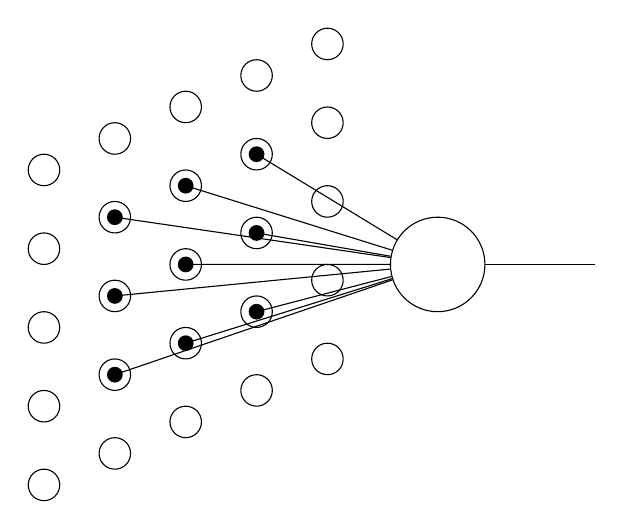
\begin{tikzpicture}
				\node[draw, circle, minimum size=1.2cm] (n) at (5,2.8) {};
				\draw (n) --  (7,2.8);
				\foreach \x in {0,1,2,3,4}
					\foreach \y in {0,1,2,3,4}
						\draw (\x*0.9+ \y*0, \x*0.4+\y*1) circle (0.2cm); %Matrixtransformation (0.7 0; 0.3 1)
				\foreach \x in {1,2,3}
					\foreach \y in {1,2,3} {
						\draw (\x*0.9+ \y*0, \x*0.4+\y*1) -- (n);
						\fill (\x*0.9+ \y*0, \x*0.4+\y*1) circle (0.1cm);
					}
			\end{tikzpicture}
	\caption{Neuron of a Convolutional Neural Network (own figure)} \label{fig:cnnneuron}
\end{figure}
\par 
For better understanding, convolution, stride, and padding are illustrated in the following paragraphs. 
\paragraph{Convolution}For example, consider the case of a grayscale image represented as one channel $X$, a kernel $K$, and an identity activation function $\varphi$. Then, the output of a convolutional neuron is computed by laying the kernel on top of the channel. Each value of the activation map is computed by multiplying the overlapping values. The resulting values are summed. The sum is processed by the activation function. In this case, the activation function is the identity function. Thus, the result is the sum itself. The activation map $Y$ is computed by sliding the kernel over each row and each column by the factor of stride. This is illustrated in Figure \ref{fig:conv}.\autocite{Goodfellow.2016}
\begin{figure}[H]
	\centering
	\ac{CNN}s are neural networks using convolutional layers. Convolutional layers are designed to input multidimensional arrays and output multidimensional arrays. 
%
For image classification, the input is composed of one or more two-dimensional arrays called channels. The channels share the same shape $w_{in} \times h_{in}$.
Consequently, the input can be represented as a three-dimensional array of shape $w_{in} \times h_{in} \times d_{in}$ with $d_{in}$ being the number of channels.
%
The output is composed of one or more two-dimensional arrays called feature maps. The feature maps share the same shape $w_{out} \times h_{out}$. Consequently, the output can be represented as a three-dimensional array of shape $w_{out} \times h_{out} \times d_{out}$ with $d_{out}$ being the number of feature maps. \autocites{LeCun.2015b}{LeCun.1998}
This is illustrated in Figure \ref{fig:cnnlayer}.
\begin{figure}[H]
	\centering
	%\cube{x offset}{y offset}{width}{height}{depth}{color}{fillcolor}

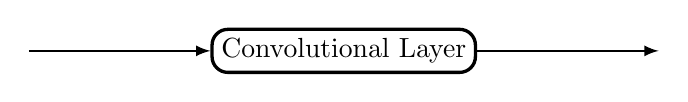
\begin{tikzpicture}[
cell/.style={
	rectangle, 
	rounded corners=2mm, 
	draw,
	very thick,
	align=center,
},
ArrowC1/.style={% Arrows with rounded corners
	rounded corners=.25cm,
	thick,
},
]
\cube{0}{0}{1}{4}{4}{black}{gray}
\node[cell] (layer) at (4,-2,-2) {Convolutional Layer};
\cube{9}{0}{1}{4}{4}{black}{gray}

\draw[-latex,ArrowC1] (0,-2,-2) -- (layer);
\draw[-latex,ArrowC1] (layer) -- (8,-2,-2);

\end{tikzpicture}
	\caption{Convolutional Layer (own figure)} \label{fig:cnnlayer}
\end{figure}
\par
Convolutional layers consist of neurons which only connect to a small region of the layer's input, see Figure \ref{fig:cnnneuron}. This region is called receptive field\autocite{LeCun.1998}. Within a receptive field, each connection of a neuron is connected to one element of the input. Consequently, a receptive field can be seen as an array slice of the layer's input. This array is of shape $k \times k \times d$.
The set of weights of a convolutional neuron's connections is referred to as filter or kernel.
The kernel can be represented as a three-dimensional array of shape $k \times k \times d$. $k$ is the size of the kernel. \autocites{Rawat.2017}{LeCun.2015b}
\par
A convolutional layer holds one neuron for each receptive field and for each kernel. This means, neurons of the same kernel share the same weights. On that account, neurons of the same kernel can be seen as $r$ copies of a neuron connected to all receptive fields or applying the same neuron to each receptive field. Applying the same neuron to each receptive field can be imagined as sliding the neuron over the input. The output of a neuron is computed as described in Section \ref{sec:neuralnetwork}. Given the input $X$, a kernel $K$, and the receptive field $X[i:i+k, j:j+k]$, the output of a neuron $y$ is computed as defined by Equation \eqref{eq:convneuron}. As a result, the output of all neurons of a kernel is computed by computing the output for all receptive fields with $i \in \{x|x_0=0, x \le w-k, x_{n+1} = x_n+stride\}$ and $j \in \{x|x_0=0, x \le h-k, _{n+1} = x_n+stride\}$. This computation loosely relates to discrete convolution. For this reason, \ac{CNN}s are called convolutional. The resulting output is a feature map. Hence, the output of a convolutional layer is computed by computing all feature maps. Derived from this, the shape of the output is $\frac{w-k+2 \cdot padding}{stride}+1 \times \frac{h-k+2 \cdot padding}{stride}+1 \times k$. Padding can be described as increasing  the input's width and height by $padding$ on both sides by filling with zeros. Imagining sliding the neuron over the input, $stride$ is the step size by which the neuron is slid. \autocite{Goodfellow.2016}
\begin{equation}
	\label{eq:convneuron}
	y = \varphi(\sum X[i:i+k, j:j+k] \cdot K)
\end{equation}
\begin{figure}[H]
	\centering
	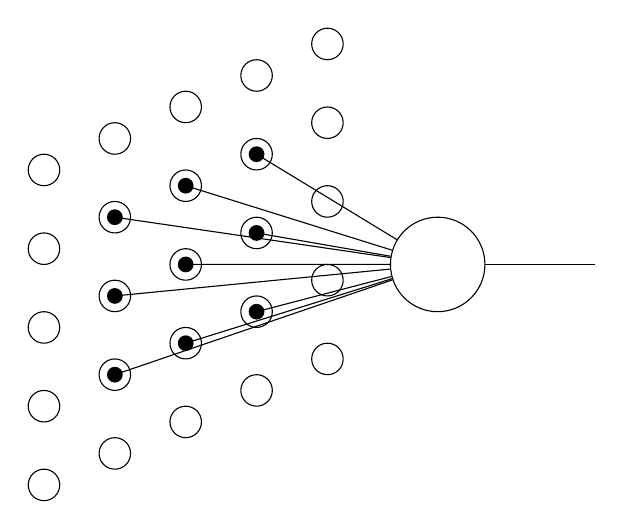
\begin{tikzpicture}
				\node[draw, circle, minimum size=1.2cm] (n) at (5,2.8) {};
				\draw (n) --  (7,2.8);
				\foreach \x in {0,1,2,3,4}
					\foreach \y in {0,1,2,3,4}
						\draw (\x*0.9+ \y*0, \x*0.4+\y*1) circle (0.2cm); %Matrixtransformation (0.7 0; 0.3 1)
				\foreach \x in {1,2,3}
					\foreach \y in {1,2,3} {
						\draw (\x*0.9+ \y*0, \x*0.4+\y*1) -- (n);
						\fill (\x*0.9+ \y*0, \x*0.4+\y*1) circle (0.1cm);
					}
			\end{tikzpicture}
	\caption{Neuron of a Convolutional Neural Network (own figure)} \label{fig:cnnneuron}
\end{figure}
\par 
For better understanding, convolution, stride, and padding are illustrated in the following paragraphs. 
\paragraph{Convolution}For example, consider the case of a grayscale image represented as one channel $X$, a kernel $K$, and an identity activation function $\varphi$. Then, the output of a convolutional neuron is computed by laying the kernel on top of the channel. Each value of the activation map is computed by multiplying the overlapping values. The resulting values are summed. The sum is processed by the activation function. In this case, the activation function is the identity function. Thus, the result is the sum itself. The activation map $Y$ is computed by sliding the kernel over each row and each column by the factor of stride. This is illustrated in Figure \ref{fig:conv}.\autocite{Goodfellow.2016}
\begin{figure}[H]
	\centering
	\ac{CNN}s are neural networks using convolutional layers. Convolutional layers are designed to input multidimensional arrays and output multidimensional arrays. 
%
For image classification, the input is composed of one or more two-dimensional arrays called channels. The channels share the same shape $w_{in} \times h_{in}$.
Consequently, the input can be represented as a three-dimensional array of shape $w_{in} \times h_{in} \times d_{in}$ with $d_{in}$ being the number of channels.
%
The output is composed of one or more two-dimensional arrays called feature maps. The feature maps share the same shape $w_{out} \times h_{out}$. Consequently, the output can be represented as a three-dimensional array of shape $w_{out} \times h_{out} \times d_{out}$ with $d_{out}$ being the number of feature maps. \autocites{LeCun.2015b}{LeCun.1998}
This is illustrated in Figure \ref{fig:cnnlayer}.
\begin{figure}[H]
	\centering
	\input{img/cnn_layer}
	\caption{Convolutional Layer (own figure)} \label{fig:cnnlayer}
\end{figure}
\par
Convolutional layers consist of neurons which only connect to a small region of the layer's input, see Figure \ref{fig:cnnneuron}. This region is called receptive field\autocite{LeCun.1998}. Within a receptive field, each connection of a neuron is connected to one element of the input. Consequently, a receptive field can be seen as an array slice of the layer's input. This array is of shape $k \times k \times d$.
The set of weights of a convolutional neuron's connections is referred to as filter or kernel.
The kernel can be represented as a three-dimensional array of shape $k \times k \times d$. $k$ is the size of the kernel. \autocites{Rawat.2017}{LeCun.2015b}
\par
A convolutional layer holds one neuron for each receptive field and for each kernel. This means, neurons of the same kernel share the same weights. On that account, neurons of the same kernel can be seen as $r$ copies of a neuron connected to all receptive fields or applying the same neuron to each receptive field. Applying the same neuron to each receptive field can be imagined as sliding the neuron over the input. The output of a neuron is computed as described in Section \ref{sec:neuralnetwork}. Given the input $X$, a kernel $K$, and the receptive field $X[i:i+k, j:j+k]$, the output of a neuron $y$ is computed as defined by Equation \eqref{eq:convneuron}. As a result, the output of all neurons of a kernel is computed by computing the output for all receptive fields with $i \in \{x|x_0=0, x \le w-k, x_{n+1} = x_n+stride\}$ and $j \in \{x|x_0=0, x \le h-k, _{n+1} = x_n+stride\}$. This computation loosely relates to discrete convolution. For this reason, \ac{CNN}s are called convolutional. The resulting output is a feature map. Hence, the output of a convolutional layer is computed by computing all feature maps. Derived from this, the shape of the output is $\frac{w-k+2 \cdot padding}{stride}+1 \times \frac{h-k+2 \cdot padding}{stride}+1 \times k$. Padding can be described as increasing  the input's width and height by $padding$ on both sides by filling with zeros. Imagining sliding the neuron over the input, $stride$ is the step size by which the neuron is slid. \autocite{Goodfellow.2016}
\begin{equation}
	\label{eq:convneuron}
	y = \varphi(\sum X[i:i+k, j:j+k] \cdot K)
\end{equation}
\begin{figure}[H]
	\centering
	\input{img/cnn_neuron}
	\caption{Neuron of a Convolutional Neural Network (own figure)} \label{fig:cnnneuron}
\end{figure}
\par 
For better understanding, convolution, stride, and padding are illustrated in the following paragraphs. 
\paragraph{Convolution}For example, consider the case of a grayscale image represented as one channel $X$, a kernel $K$, and an identity activation function $\varphi$. Then, the output of a convolutional neuron is computed by laying the kernel on top of the channel. Each value of the activation map is computed by multiplying the overlapping values. The resulting values are summed. The sum is processed by the activation function. In this case, the activation function is the identity function. Thus, the result is the sum itself. The activation map $Y$ is computed by sliding the kernel over each row and each column by the factor of stride. This is illustrated in Figure \ref{fig:conv}.\autocite{Goodfellow.2016}
\begin{figure}[H]
	\centering
	\input{img/conv}
	\caption{Convolution Illustration (own figure)} \label{fig:conv}
\end{figure}
\paragraph{Stride} For example, consider the case of a grayscale image represented as one channel~$X$, a kernel~$K$, and a $stride$~of~$1$ and~$2$ respectively. A stride~of~$1$ means sliding the kernel with a step~size~of~$1$. A stride~of~$2$ means sliding the kernel with a step~size~of~$2$. This is illustrated in Figure~\ref{fig:stride}.\autocite{Goodfellow.2016}
\begin{figure}[H]
	\centering
	\input{img/stride}
	\caption{Stride Illustration (own figure)} \label{fig:stride}
\end{figure}
\paragraph{Padding} For example, consider the case of a grayscale image represented as one channel $X$ and a $padding$ of $1$. A padding of $1$ adds $1$ row and column of $0$s respectively to each edge of the channel. This is illustrated in Figure \ref{fig:padding}.\autocite{Goodfellow.2016}
\begin{figure}[H]
	\centering
	\input{img/padding}
	\caption{Padding Illustration (own figure)} \label{fig:padding}
\end{figure}
\par
The best-performing \ac{CNN} found in the course of the literature review is the 19-layer version of \cite{Simonyan.2014}'s VGG, called VGG-19.
The input of VGG-19 is a $224$-by-$224$-pixel, \ac{RGB} image. The output of VGG-19 comprises the probabilities of the $c$ target classes. 
VGG-19 is comprised of 16 convolutional layers and 3 dense layers.
All layers except the output layer use the \ac{ReLU} activation function. The output layer uses the softmax activation function.
The convolutional layers have different numbers of kernels. The kernels are of kernel size $3$.
Max pooling is applied after layer number $2$, $4$, $8$, $12$, and $16$. The pooling size is $2$ and the pooling stride is $2$.
For each layer, the number of kernels and neurons respectively are outlined in Table \ref{tab:vgg}. \autocite{Simonyan.2014}
\begin{xltabular}{\textwidth}{lXl}\toprule
	\caption{VGG-19 Configuration} \label{tab:vgg}\\
	\textbf{Layer Number} & \textbf{Layer} & \textbf{Number of Neurons/Kernels} \\\midrule \endhead
	$1$ & Convolutional Layer & $64$\\\midrule
	$2$ & Convolutional Layer & $64$\\\midrule
	$3$ & Convolutional Layer & $128$\\\midrule
	$4$ & Convolutional Layer & $128$\\\midrule
	$5$ & Convolutional Layer & $256$\\\midrule
	$6$ & Convolutional Layer & $256$\\\midrule
	$7$ & Convolutional Layer & $256$\\\midrule
	$8$ & Convolutional Layer & $256$\\\midrule
	$9$ & Convolutional Layer & $512$\\\midrule
	$10$ & Convolutional Layer & $512$\\\midrule
	$11$ & Convolutional Layer & $512$\\\midrule
	$12$ & Convolutional Layer & $512$\\\midrule
	$13$ & Convolutional Layer & $512$\\\midrule
	$14$ & Convolutional Layer & $512$\\\midrule
	$15$ & Convolutional Layer & $512$\\\midrule
	$16$ & Convolutional Layer & $512$\\\midrule
	$17$ & Dense Layer & $4096$\\\midrule
	$18$ & Dense Layer & $4096$\\\midrule
	$19$ & Dense Layer & $c$
	\\\bottomrule
\end{xltabular}
%preprocessing subtracting mean rgb of training set
	\caption{Convolution Illustration (own figure)} \label{fig:conv}
\end{figure}
\paragraph{Stride} For example, consider the case of a grayscale image represented as one channel~$X$, a kernel~$K$, and a $stride$~of~$1$ and~$2$ respectively. A stride~of~$1$ means sliding the kernel with a step~size~of~$1$. A stride~of~$2$ means sliding the kernel with a step~size~of~$2$. This is illustrated in Figure~\ref{fig:stride}.\autocite{Goodfellow.2016}
\begin{figure}[H]
	\centering
	\begin{tikzpicture}
\matrix (mtr) [matrix of nodes,row sep=-\pgflinewidth, nodes={draw}]
{
	|[fill=orange!10]|0 & |[fill=orange!40]|1 & |[fill=orange!70]|0 & |[fill=orange!70]|1 & |[fill=orange!70]|0 & 0 & 0 & 0 & 0\\
	|[fill=orange!10]|0 & |[fill=orange!40]|0 & |[fill=orange!70]|1 & |[fill=orange!70]|1 & |[fill=orange!70]|1 & 0 & 0 & 1 & 0\\
	|[fill=orange!10]|1 & |[fill=orange!40]|0 & |[fill=orange!70]|0 & |[fill=orange!70]|1 & |[fill=orange!70]|1 & 1 & 0 & 1 & 0\\
	0 & 0 & 0 & 0 & 1 & 0 & 0 & 0 & 0\\
	0 & 0 & 1 & 1 & 0 & 1 & 0 & 0 & 1\\
	0 & 1 & 1 & 1 & 0 & 1 & 1 & 0 & 1\\
	0 & 1 & 1 & 0 & 0 & 0 & 1 & 1 & 0\\
};

\node [below= of mtr-5-5.south] (lm) {$stride = 1$};

\matrix (mt) [matrix of nodes,row sep=-\pgflinewidth, nodes={draw}, right = 4em of mtr]
{
	|[fill=orange!10]|0 & |[fill=orange!10]|1 & |[fill=orange!40]|0 & |[fill=orange!40]|1 & |[fill=orange!70]|0 & |[fill=orange!70]|0 & |[fill=orange!70]|0 & 0 & 0\\
	|[fill=orange!10]|0 & |[fill=orange!10]|0 & |[fill=orange!40]|1 & |[fill=orange!40]|1 & |[fill=orange!70]|1 & |[fill=orange!70]|0 & |[fill=orange!70]|0 & 1 & 0\\
	|[fill=orange!10]|1 & |[fill=orange!10]|0 & |[fill=orange!40]|0 & |[fill=orange!40]|1 & |[fill=orange!70]|1 & |[fill=orange!70]|1 & |[fill=orange!70]|0 & 1 & 0\\
	0 & 0 & 0 & 0 & 1 & 0 & 0 & 0 & 0\\
	0 & 0 & 1 & 1 & 0 & 1 & 0 & 0 & 1\\
	0 & 1 & 1 & 1 & 0 & 1 & 1 & 0 & 1\\
	0 & 1 & 1 & 0 & 0 & 0 & 1 & 1 & 0\\
};

\node [below= of mt-5-5.south] (m) {$stride = 2$};

\end{tikzpicture}
	\caption{Stride Illustration (own figure)} \label{fig:stride}
\end{figure}
\paragraph{Padding} For example, consider the case of a grayscale image represented as one channel $X$ and a $padding$ of $1$. A padding of $1$ adds $1$ row and column of $0$s respectively to each edge of the channel. This is illustrated in Figure \ref{fig:padding}.\autocite{Goodfellow.2016}
\begin{figure}[H]
	\centering
	\begin{tikzpicture}
\matrix (mtr) [matrix of nodes,row sep=-\pgflinewidth, nodes={draw}]
{
	0 & 1 & 0 & 1 & 0 & 0 & 0 & 0 & 0\\
	0 & 0 & 1 & 1 & 1 & 0 & 0 & 1 & 0\\
	1 & 0 & 0 & 1 & 1 & 1 & 0 & 1 & 0\\
	0 & 0 & 0 & 0 & 1 & 0 & 0 & 0 & 0\\
	0 & 0 & 1 & 1 & 0 & 1 & 0 & 0 & 1\\
	0 & 1 & 1 & 1 & 0 & 1 & 1 & 0 & 1\\
	0 & 1 & 1 & 0 & 0 & 0 & 1 & 1 & 0\\
};

\node [below= of mtr-6-5.south] (lm) {$X$};

\matrix (mt) [matrix of nodes,row sep=-\pgflinewidth, nodes={draw}, right = 4em of mtr]
{
	|[fill=blue!30]|0 & |[fill=blue!30]|0 & |[fill=blue!30]|0 & |[fill=blue!30]|0 & |[fill=blue!30]|0 & |[fill=blue!30]|0 & |[fill=blue!30]|0 & |[fill=blue!30]|0 & |[fill=blue!30]|0 & |[fill=blue!30]|0 & |[fill=blue!30]|0\\
	|[fill=blue!30]|0 & 0 & 1 & 0 & 1 & 0 & 0 & 0 & 0 & 0 & |[fill=blue!30]|0\\
	|[fill=blue!30]|0 & 0 & 0 & 1 & 1 & 1 & 0 & 0 & 1 & 0 & |[fill=blue!30]|0\\
	|[fill=blue!30]|0 & 1 & 0 & 0 & 1 & 1 & 1 & 0 & 1 & 0 & |[fill=blue!30]|0\\	
	|[fill=blue!30]|0 & 0 & 0 & 0 & 0 & 1 & 0 & 0 & 0 & 0 & |[fill=blue!30]|0\\
	|[fill=blue!30]|0 & 0 & 0 & 1 & 1 & 0 & 1 & 0 & 0 & 1 & |[fill=blue!30]|0\\
	|[fill=blue!30]|0 & 0 & 1 & 1 & 1 & 0 & 1 & 1 & 0 & 1 & |[fill=blue!30]|0\\
	|[fill=blue!30]|0 & 0 & 1 & 1 & 0 & 0 & 0 & 1 & 1 & 0 & |[fill=blue!30]|0\\
	|[fill=blue!30]|0 & |[fill=blue!30]|0 & |[fill=blue!30]|0 & |[fill=blue!30]|0 & |[fill=blue!30]|0 & |[fill=blue!30]|0 & |[fill=blue!30]|0 & |[fill=blue!30]|0 & |[fill=blue!30]|0 & |[fill=blue!30]|0 & |[fill=blue!30]|0\\
};

\node [below= of mt-7-6.south] (m) {$X$ with $padding$ of $1$};

\end{tikzpicture}
	\caption{Padding Illustration (own figure)} \label{fig:padding}
\end{figure}
\par
The best-performing \ac{CNN} found in the course of the literature review is the 19-layer version of \cite{Simonyan.2014}'s VGG, called VGG-19.
The input of VGG-19 is a $224$-by-$224$-pixel, \ac{RGB} image. The output of VGG-19 comprises the probabilities of the $c$ target classes. 
VGG-19 is comprised of 16 convolutional layers and 3 dense layers.
All layers except the output layer use the \ac{ReLU} activation function. The output layer uses the softmax activation function.
The convolutional layers have different numbers of kernels. The kernels are of kernel size $3$.
Max pooling is applied after layer number $2$, $4$, $8$, $12$, and $16$. The pooling size is $2$ and the pooling stride is $2$.
For each layer, the number of kernels and neurons respectively are outlined in Table \ref{tab:vgg}. \autocite{Simonyan.2014}
\begin{xltabular}{\textwidth}{lXl}\toprule
	\caption{VGG-19 Configuration} \label{tab:vgg}\\
	\textbf{Layer Number} & \textbf{Layer} & \textbf{Number of Neurons/Kernels} \\\midrule \endhead
	$1$ & Convolutional Layer & $64$\\\midrule
	$2$ & Convolutional Layer & $64$\\\midrule
	$3$ & Convolutional Layer & $128$\\\midrule
	$4$ & Convolutional Layer & $128$\\\midrule
	$5$ & Convolutional Layer & $256$\\\midrule
	$6$ & Convolutional Layer & $256$\\\midrule
	$7$ & Convolutional Layer & $256$\\\midrule
	$8$ & Convolutional Layer & $256$\\\midrule
	$9$ & Convolutional Layer & $512$\\\midrule
	$10$ & Convolutional Layer & $512$\\\midrule
	$11$ & Convolutional Layer & $512$\\\midrule
	$12$ & Convolutional Layer & $512$\\\midrule
	$13$ & Convolutional Layer & $512$\\\midrule
	$14$ & Convolutional Layer & $512$\\\midrule
	$15$ & Convolutional Layer & $512$\\\midrule
	$16$ & Convolutional Layer & $512$\\\midrule
	$17$ & Dense Layer & $4096$\\\midrule
	$18$ & Dense Layer & $4096$\\\midrule
	$19$ & Dense Layer & $c$
	\\\bottomrule
\end{xltabular}
%preprocessing subtracting mean rgb of training set
	\caption{Convolution Illustration (own figure)} \label{fig:conv}
\end{figure}
\paragraph{Stride} For example, consider the case of a grayscale image represented as one channel~$X$, a kernel~$K$, and a $stride$~of~$1$ and~$2$ respectively. A stride~of~$1$ means sliding the kernel with a step~size~of~$1$. A stride~of~$2$ means sliding the kernel with a step~size~of~$2$. This is illustrated in Figure~\ref{fig:stride}.\autocite{Goodfellow.2016}
\begin{figure}[H]
	\centering
	\begin{tikzpicture}
\matrix (mtr) [matrix of nodes,row sep=-\pgflinewidth, nodes={draw}]
{
	|[fill=orange!10]|0 & |[fill=orange!40]|1 & |[fill=orange!70]|0 & |[fill=orange!70]|1 & |[fill=orange!70]|0 & 0 & 0 & 0 & 0\\
	|[fill=orange!10]|0 & |[fill=orange!40]|0 & |[fill=orange!70]|1 & |[fill=orange!70]|1 & |[fill=orange!70]|1 & 0 & 0 & 1 & 0\\
	|[fill=orange!10]|1 & |[fill=orange!40]|0 & |[fill=orange!70]|0 & |[fill=orange!70]|1 & |[fill=orange!70]|1 & 1 & 0 & 1 & 0\\
	0 & 0 & 0 & 0 & 1 & 0 & 0 & 0 & 0\\
	0 & 0 & 1 & 1 & 0 & 1 & 0 & 0 & 1\\
	0 & 1 & 1 & 1 & 0 & 1 & 1 & 0 & 1\\
	0 & 1 & 1 & 0 & 0 & 0 & 1 & 1 & 0\\
};

\node [below= of mtr-5-5.south] (lm) {$stride = 1$};

\matrix (mt) [matrix of nodes,row sep=-\pgflinewidth, nodes={draw}, right = 4em of mtr]
{
	|[fill=orange!10]|0 & |[fill=orange!10]|1 & |[fill=orange!40]|0 & |[fill=orange!40]|1 & |[fill=orange!70]|0 & |[fill=orange!70]|0 & |[fill=orange!70]|0 & 0 & 0\\
	|[fill=orange!10]|0 & |[fill=orange!10]|0 & |[fill=orange!40]|1 & |[fill=orange!40]|1 & |[fill=orange!70]|1 & |[fill=orange!70]|0 & |[fill=orange!70]|0 & 1 & 0\\
	|[fill=orange!10]|1 & |[fill=orange!10]|0 & |[fill=orange!40]|0 & |[fill=orange!40]|1 & |[fill=orange!70]|1 & |[fill=orange!70]|1 & |[fill=orange!70]|0 & 1 & 0\\
	0 & 0 & 0 & 0 & 1 & 0 & 0 & 0 & 0\\
	0 & 0 & 1 & 1 & 0 & 1 & 0 & 0 & 1\\
	0 & 1 & 1 & 1 & 0 & 1 & 1 & 0 & 1\\
	0 & 1 & 1 & 0 & 0 & 0 & 1 & 1 & 0\\
};

\node [below= of mt-5-5.south] (m) {$stride = 2$};

\end{tikzpicture}
	\caption{Stride Illustration (own figure)} \label{fig:stride}
\end{figure}
\paragraph{Padding} For example, consider the case of a grayscale image represented as one channel $X$ and a $padding$ of $1$. A padding of $1$ adds $1$ row and column of $0$s respectively to each edge of the channel. This is illustrated in Figure \ref{fig:padding}.\autocite{Goodfellow.2016}
\begin{figure}[H]
	\centering
	\begin{tikzpicture}
\matrix (mtr) [matrix of nodes,row sep=-\pgflinewidth, nodes={draw}]
{
	0 & 1 & 0 & 1 & 0 & 0 & 0 & 0 & 0\\
	0 & 0 & 1 & 1 & 1 & 0 & 0 & 1 & 0\\
	1 & 0 & 0 & 1 & 1 & 1 & 0 & 1 & 0\\
	0 & 0 & 0 & 0 & 1 & 0 & 0 & 0 & 0\\
	0 & 0 & 1 & 1 & 0 & 1 & 0 & 0 & 1\\
	0 & 1 & 1 & 1 & 0 & 1 & 1 & 0 & 1\\
	0 & 1 & 1 & 0 & 0 & 0 & 1 & 1 & 0\\
};

\node [below= of mtr-6-5.south] (lm) {$X$};

\matrix (mt) [matrix of nodes,row sep=-\pgflinewidth, nodes={draw}, right = 4em of mtr]
{
	|[fill=blue!30]|0 & |[fill=blue!30]|0 & |[fill=blue!30]|0 & |[fill=blue!30]|0 & |[fill=blue!30]|0 & |[fill=blue!30]|0 & |[fill=blue!30]|0 & |[fill=blue!30]|0 & |[fill=blue!30]|0 & |[fill=blue!30]|0 & |[fill=blue!30]|0\\
	|[fill=blue!30]|0 & 0 & 1 & 0 & 1 & 0 & 0 & 0 & 0 & 0 & |[fill=blue!30]|0\\
	|[fill=blue!30]|0 & 0 & 0 & 1 & 1 & 1 & 0 & 0 & 1 & 0 & |[fill=blue!30]|0\\
	|[fill=blue!30]|0 & 1 & 0 & 0 & 1 & 1 & 1 & 0 & 1 & 0 & |[fill=blue!30]|0\\	
	|[fill=blue!30]|0 & 0 & 0 & 0 & 0 & 1 & 0 & 0 & 0 & 0 & |[fill=blue!30]|0\\
	|[fill=blue!30]|0 & 0 & 0 & 1 & 1 & 0 & 1 & 0 & 0 & 1 & |[fill=blue!30]|0\\
	|[fill=blue!30]|0 & 0 & 1 & 1 & 1 & 0 & 1 & 1 & 0 & 1 & |[fill=blue!30]|0\\
	|[fill=blue!30]|0 & 0 & 1 & 1 & 0 & 0 & 0 & 1 & 1 & 0 & |[fill=blue!30]|0\\
	|[fill=blue!30]|0 & |[fill=blue!30]|0 & |[fill=blue!30]|0 & |[fill=blue!30]|0 & |[fill=blue!30]|0 & |[fill=blue!30]|0 & |[fill=blue!30]|0 & |[fill=blue!30]|0 & |[fill=blue!30]|0 & |[fill=blue!30]|0 & |[fill=blue!30]|0\\
};

\node [below= of mt-7-6.south] (m) {$X$ with $padding$ of $1$};

\end{tikzpicture}
	\caption{Padding Illustration (own figure)} \label{fig:padding}
\end{figure}
\par
The best-performing \ac{CNN} found in the course of the literature review is the 19-layer version of \cite{Simonyan.2014}'s VGG, called VGG-19.
The input of VGG-19 is a $224$-by-$224$-pixel, \ac{RGB} image. The output of VGG-19 comprises the probabilities of the $c$ target classes. 
VGG-19 is comprised of 16 convolutional layers and 3 dense layers.
All layers except the output layer use the \ac{ReLU} activation function. The output layer uses the softmax activation function.
The convolutional layers have different numbers of kernels. The kernels are of kernel size $3$.
Max pooling is applied after layer number $2$, $4$, $8$, $12$, and $16$. The pooling size is $2$ and the pooling stride is $2$.
For each layer, the number of kernels and neurons respectively are outlined in Table \ref{tab:vgg}. \autocite{Simonyan.2014}
\begin{xltabular}{\textwidth}{lXl}\toprule
	\caption{VGG-19 Configuration} \label{tab:vgg}\\
	\textbf{Layer Number} & \textbf{Layer} & \textbf{Number of Neurons/Kernels} \\\midrule \endhead
	$1$ & Convolutional Layer & $64$\\\midrule
	$2$ & Convolutional Layer & $64$\\\midrule
	$3$ & Convolutional Layer & $128$\\\midrule
	$4$ & Convolutional Layer & $128$\\\midrule
	$5$ & Convolutional Layer & $256$\\\midrule
	$6$ & Convolutional Layer & $256$\\\midrule
	$7$ & Convolutional Layer & $256$\\\midrule
	$8$ & Convolutional Layer & $256$\\\midrule
	$9$ & Convolutional Layer & $512$\\\midrule
	$10$ & Convolutional Layer & $512$\\\midrule
	$11$ & Convolutional Layer & $512$\\\midrule
	$12$ & Convolutional Layer & $512$\\\midrule
	$13$ & Convolutional Layer & $512$\\\midrule
	$14$ & Convolutional Layer & $512$\\\midrule
	$15$ & Convolutional Layer & $512$\\\midrule
	$16$ & Convolutional Layer & $512$\\\midrule
	$17$ & Dense Layer & $4096$\\\midrule
	$18$ & Dense Layer & $4096$\\\midrule
	$19$ & Dense Layer & $c$
	\\\bottomrule
\end{xltabular}
%preprocessing subtracting mean rgb of training set
	\caption{Convolution Illustration (own figure)} \label{fig:conv}
\end{figure}
\paragraph{Stride} For example, consider the case of a grayscale image represented as one channel~$X$, a kernel~$K$, and a $stride$~of~$1$ and~$2$ respectively. A stride~of~$1$ means sliding the kernel with a step~size~of~$1$. A stride~of~$2$ means sliding the kernel with a step~size~of~$2$. This is illustrated in Figure~\ref{fig:stride}.\autocite{Goodfellow.2016}
\begin{figure}[H]
	\centering
	\begin{tikzpicture}
\matrix (mtr) [matrix of nodes,row sep=-\pgflinewidth, nodes={draw}]
{
	|[fill=orange!10]|0 & |[fill=orange!40]|1 & |[fill=orange!70]|0 & |[fill=orange!70]|1 & |[fill=orange!70]|0 & 0 & 0 & 0 & 0\\
	|[fill=orange!10]|0 & |[fill=orange!40]|0 & |[fill=orange!70]|1 & |[fill=orange!70]|1 & |[fill=orange!70]|1 & 0 & 0 & 1 & 0\\
	|[fill=orange!10]|1 & |[fill=orange!40]|0 & |[fill=orange!70]|0 & |[fill=orange!70]|1 & |[fill=orange!70]|1 & 1 & 0 & 1 & 0\\
	0 & 0 & 0 & 0 & 1 & 0 & 0 & 0 & 0\\
	0 & 0 & 1 & 1 & 0 & 1 & 0 & 0 & 1\\
	0 & 1 & 1 & 1 & 0 & 1 & 1 & 0 & 1\\
	0 & 1 & 1 & 0 & 0 & 0 & 1 & 1 & 0\\
};

\node [below= of mtr-5-5.south] (lm) {$stride = 1$};

\matrix (mt) [matrix of nodes,row sep=-\pgflinewidth, nodes={draw}, right = 4em of mtr]
{
	|[fill=orange!10]|0 & |[fill=orange!10]|1 & |[fill=orange!40]|0 & |[fill=orange!40]|1 & |[fill=orange!70]|0 & |[fill=orange!70]|0 & |[fill=orange!70]|0 & 0 & 0\\
	|[fill=orange!10]|0 & |[fill=orange!10]|0 & |[fill=orange!40]|1 & |[fill=orange!40]|1 & |[fill=orange!70]|1 & |[fill=orange!70]|0 & |[fill=orange!70]|0 & 1 & 0\\
	|[fill=orange!10]|1 & |[fill=orange!10]|0 & |[fill=orange!40]|0 & |[fill=orange!40]|1 & |[fill=orange!70]|1 & |[fill=orange!70]|1 & |[fill=orange!70]|0 & 1 & 0\\
	0 & 0 & 0 & 0 & 1 & 0 & 0 & 0 & 0\\
	0 & 0 & 1 & 1 & 0 & 1 & 0 & 0 & 1\\
	0 & 1 & 1 & 1 & 0 & 1 & 1 & 0 & 1\\
	0 & 1 & 1 & 0 & 0 & 0 & 1 & 1 & 0\\
};

\node [below= of mt-5-5.south] (m) {$stride = 2$};

\end{tikzpicture}
	\caption{Stride Illustration (own figure)} \label{fig:stride}
\end{figure}
\paragraph{Padding} For example, consider the case of a grayscale image represented as one channel $X$ and a $padding$ of $1$. A padding of $1$ adds $1$ row and column of $0$s respectively to each edge of the channel. This is illustrated in Figure \ref{fig:padding}.\autocite{Goodfellow.2016}
\begin{figure}[H]
	\centering
	\begin{tikzpicture}
\matrix (mtr) [matrix of nodes,row sep=-\pgflinewidth, nodes={draw}]
{
	0 & 1 & 0 & 1 & 0 & 0 & 0 & 0 & 0\\
	0 & 0 & 1 & 1 & 1 & 0 & 0 & 1 & 0\\
	1 & 0 & 0 & 1 & 1 & 1 & 0 & 1 & 0\\
	0 & 0 & 0 & 0 & 1 & 0 & 0 & 0 & 0\\
	0 & 0 & 1 & 1 & 0 & 1 & 0 & 0 & 1\\
	0 & 1 & 1 & 1 & 0 & 1 & 1 & 0 & 1\\
	0 & 1 & 1 & 0 & 0 & 0 & 1 & 1 & 0\\
};

\node [below= of mtr-6-5.south] (lm) {$X$};

\matrix (mt) [matrix of nodes,row sep=-\pgflinewidth, nodes={draw}, right = 4em of mtr]
{
	|[fill=blue!30]|0 & |[fill=blue!30]|0 & |[fill=blue!30]|0 & |[fill=blue!30]|0 & |[fill=blue!30]|0 & |[fill=blue!30]|0 & |[fill=blue!30]|0 & |[fill=blue!30]|0 & |[fill=blue!30]|0 & |[fill=blue!30]|0 & |[fill=blue!30]|0\\
	|[fill=blue!30]|0 & 0 & 1 & 0 & 1 & 0 & 0 & 0 & 0 & 0 & |[fill=blue!30]|0\\
	|[fill=blue!30]|0 & 0 & 0 & 1 & 1 & 1 & 0 & 0 & 1 & 0 & |[fill=blue!30]|0\\
	|[fill=blue!30]|0 & 1 & 0 & 0 & 1 & 1 & 1 & 0 & 1 & 0 & |[fill=blue!30]|0\\	
	|[fill=blue!30]|0 & 0 & 0 & 0 & 0 & 1 & 0 & 0 & 0 & 0 & |[fill=blue!30]|0\\
	|[fill=blue!30]|0 & 0 & 0 & 1 & 1 & 0 & 1 & 0 & 0 & 1 & |[fill=blue!30]|0\\
	|[fill=blue!30]|0 & 0 & 1 & 1 & 1 & 0 & 1 & 1 & 0 & 1 & |[fill=blue!30]|0\\
	|[fill=blue!30]|0 & 0 & 1 & 1 & 0 & 0 & 0 & 1 & 1 & 0 & |[fill=blue!30]|0\\
	|[fill=blue!30]|0 & |[fill=blue!30]|0 & |[fill=blue!30]|0 & |[fill=blue!30]|0 & |[fill=blue!30]|0 & |[fill=blue!30]|0 & |[fill=blue!30]|0 & |[fill=blue!30]|0 & |[fill=blue!30]|0 & |[fill=blue!30]|0 & |[fill=blue!30]|0\\
};

\node [below= of mt-7-6.south] (m) {$X$ with $padding$ of $1$};

\end{tikzpicture}
	\caption{Padding Illustration (own figure)} \label{fig:padding}
\end{figure}
\par
The best-performing \ac{CNN} found in the course of the literature review is the 19-layer version of \cite{Simonyan.2014}'s VGG, called VGG-19.
The input of VGG-19 is a $224$-by-$224$-pixel, \ac{RGB} image. The output of VGG-19 comprises the probabilities of the $c$ target classes. 
VGG-19 is comprised of 16 convolutional layers and 3 dense layers.
All layers except the output layer use the \ac{ReLU} activation function. The output layer uses the softmax activation function.
The convolutional layers have different numbers of kernels. The kernels are of kernel size $3$.
Max pooling is applied after layer number $2$, $4$, $8$, $12$, and $16$. The pooling size is $2$ and the pooling stride is $2$.
For each layer, the number of kernels and neurons respectively are outlined in Table \ref{tab:vgg}. \autocite{Simonyan.2014}
\begin{xltabular}{\textwidth}{lXl}\toprule
	\caption{VGG-19 Configuration} \label{tab:vgg}\\
	\textbf{Layer Number} & \textbf{Layer} & \textbf{Number of Neurons/Kernels} \\\midrule \endhead
	$1$ & Convolutional Layer & $64$\\\midrule
	$2$ & Convolutional Layer & $64$\\\midrule
	$3$ & Convolutional Layer & $128$\\\midrule
	$4$ & Convolutional Layer & $128$\\\midrule
	$5$ & Convolutional Layer & $256$\\\midrule
	$6$ & Convolutional Layer & $256$\\\midrule
	$7$ & Convolutional Layer & $256$\\\midrule
	$8$ & Convolutional Layer & $256$\\\midrule
	$9$ & Convolutional Layer & $512$\\\midrule
	$10$ & Convolutional Layer & $512$\\\midrule
	$11$ & Convolutional Layer & $512$\\\midrule
	$12$ & Convolutional Layer & $512$\\\midrule
	$13$ & Convolutional Layer & $512$\\\midrule
	$14$ & Convolutional Layer & $512$\\\midrule
	$15$ & Convolutional Layer & $512$\\\midrule
	$16$ & Convolutional Layer & $512$\\\midrule
	$17$ & Dense Layer & $4096$\\\midrule
	$18$ & Dense Layer & $4096$\\\midrule
	$19$ & Dense Layer & $c$
	\\\bottomrule
\end{xltabular}
%preprocessing subtracting mean rgb of training set